\documentclass{article}

% Packages
\usepackage{amsmath, amssymb}   % math formatting & symbols
\usepackage{graphicx}           % insert graphics
\usepackage{listings}
%\usepackage{eulervm, bookman}   % fonts for math & symbols
\usepackage{fullpage}          % fullpage margins

\lstset{language=Matlab,
    basicstyle=\scriptsize\ttfamily,
    stringstyle=\ttfamily,
    showstringspaces=false,
    breaklines=true,
    frameround=ffff,
    frame=single,
}

\begin{document}
% Title 
\title{Math 104A: Homework 4}
\author{Raghav Thirumulu, Perm 3499720 \\ \texttt{rrajuthirumulu@umail.ucsb.edu}}
\maketitle

\begin{enumerate}
    \item % 1 
        \begin{lstlisting}
        function [a,b,c,d] = cubic_spline_coefficients(x,y)
        % Computer code for evaluating coefficients of cubic spline
        % Input:  x      --- vector of x points
        %         y      --- vector of y points
        % Output a,b,c,d --- coefficients of cubic spline
        % Author: Raghav Thirumulu, Perm 3499720
        % Date:   07/23/2018

        % Find length of our dataset
        n=length(x);

        % Find interval lengths and store in h
        for i=1:n-1
            h(i)=x(i+1)-x(i);
        end

        % Create vectors/matrices for storing values
        A=zeros(n,n);
        f=zeros(n,1);
        A(1,1)=1;
        A(n,n)=1;

        % Iterate through, replacing points
        for i=2:n-1
            A(i,i)=2*(h(i)+h(i-1));
            f(i)=6*((y(i+1)-y(i))/h(i)-(y(i)-y(i-1))/h(i-1));
        end
        for i=2:n-2
            A(i,i+1)=h(i+1);
        end
        for i=3:n-1
            A(i,i-1)=h(i);
        end

        s=A\f;

        for i=1:n-1
            a(i)=(s(i+1)-s(i))/(6*h(i));
            b(i)=s(i)/2;
            c(i)=(y(i+1)-y(i))/h(i)-(2*h(i)*s(i)+h(i)*s(i+1))/6;
            d(i)=y(i);
        end
        \end{lstlisting}
        
        \begin{lstlisting}
        function ybar = cubic_spline_eval(s0,s1,s2,s3,xbar,x)
        % Computer code for evaluating cubic spline at certain point
        % Input: s0,s1,s2,s3 --- coefficients we solved for earlier
        %        xbar        --- x value we are interpolating at
        %        x           --- data points for interpolation
        % Output ybar        --- evaluation of cubic spline
        % Author: Raghav Thirumulu, Perm 3499720
        % Date:   07/23/2018

        n=length(x);
        i=1;

        while (xbar>x(i+1) && i<=n-1)
            i=i+1;
        end

        % Multiply coefficients with degree for evaluation
        ybar=s0(i)*(xbar-x(i))^3+s1(i)*(xbar-x(i))^2+s2(i)*(xbar-x(i))+s3(i);
        \end{lstlisting}
    
    \item
        \begin{tabular}{||c c c c c c c c||} 
        \hline
         S0(t,x) & S1(t,x) & S2(t,x) & S3(t,x) & S0(t,y) & S1(t,y) & S2(t,y) & S3(t,y)  \\ [0.5ex] 
        \hline \hline
        0.0157 & 0 & -0.9769 & 1.5000 & 0.2829 & 0 & 0.1347 & 0.7500 \\ 
        \hline
        0.0320 & 0.0291 & -0.9588 & 0.9000 & -3.0574 & 0.5245 & 0.4564 & 0.9000 \\
        \hline
        1.0594 & 0.0596 & -0.9088 & 0.6000 & 2.6103 & -2.3831 & -0.1297 & 1.0000 \\
        \hline
        -2.1432 & 1.0766 & -0.4928 & 0.3500 & -0.5798 & 0.1229 & -0.8813 & 0.8000 \\
        \hline
        6.3975 & -1.3731 & -0.4653 & 0.2000 & 2.5834 & -0.5398 & -0.9711 & 0.4500 \\  
        \hline
        -3.9670 & 3.7897 & 0.0829 & 0.1000 & -0.9674 & 1.5449 & -0.7150 & 0.2000 \\
        \hline
        0.9217 & -1.1136 & 1.3086 & 0.5000 & -0.3785 & 0.3493 & 0.1164 & 0.1000 \\
        \hline
        -0.1966 & 0.2967 & 0.8946 & 1.0000 & 0.1523 & -0.2299 & 0.1765 & 0.2000 \\ [0.5ex]
        \hline
\end{tabular}
        \begin{lstlisting}
        function plot_cubic_spline(t,s0,s1,s2,s3,s4,s5,s6,s7)
        % Computer code for plotting parametric spline function
        % Input:  t            --- vector of t values for interpolation
        %         s0,s1,s2,s3  --- evaluation of coefficients from
        %         cubic_spline_coefficients(t,x)
        %         s4,s5,s6,s7  --- evaluation of coefficients from
        %         cubic_spline_coefficients(t,y)
        % Output: Plot of parametric curve of x(t) vs y(t)
        % Author: Raghav Thirumulu, Perm 3499720
        % Date:   07/23/2018
        n = length(t);

        for i=1:n-1
            xx(i) = cubic_spline_eval(s0,s1,s2,s3,t(i),t);
            yy(i) = cubic_spline_eval(s4,s5,s6,s7,t(i),t);
        end
        plot(xx,yy,'b');
        title('Parametric representation of curve'); 
        xlabel('x(t)');
        ylabel('y(t)');
        \end{lstlisting}
        \begin{center}
                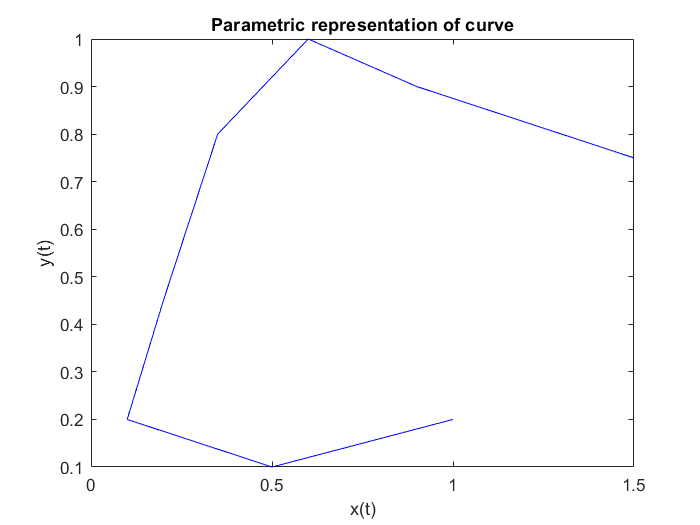
\includegraphics[scale=0.6]{parametric.png}
        \end{center}
        \end{enumerate}
\end{document}
